\documentclass[12pt,a4paper]{article}
\usepackage[T1]{fontenc}
\usepackage{amsmath,amssymb,mathrsfs,tikz,times,pifont}
\usepackage{enumitem}
\usepackage{multicol}
\usepackage{lmodern}
\usetikzlibrary{trees}
\newcommand\circitem[1]{%
\tikz[baseline=(char.base)]{
\node[circle,draw=gray, fill=red!55,
minimum size=1.2em,inner sep=0] (char) {#1};}}
\newcommand\boxitem[1]{%
\tikz[baseline=(char.base)]{
\node[fill=cyan,
minimum size=1.2em,inner sep=0] (char) {#1};}}
\setlist[enumerate,1]{label=\protect\circitem{\arabic*}}
\setlist[enumerate,2]{label=\protect\boxitem{\alph*}}
%%%::::::by chnini ameur :::::::%%%
\everymath{\displaystyle}
\usepackage[left=1cm,right=1cm,top=1cm,bottom=1.7cm]{geometry}
\usepackage[colorlinks=true, linkcolor=blue, urlcolor=blue, citecolor=blue]{hyperref}
\usepackage{array,multirow}
\usepackage[most]{tcolorbox}
\usepackage{varwidth}
\usepackage{float} %pour utiliser l'option [H] qui force l'image à apparaître exactement à l'endroit où elle est placée dans le code.
\tcbuselibrary{skins,hooks}
\usetikzlibrary{patterns}
%%%::::::by chnini ameur :::::::%%%
\newtcolorbox{exa}[2][]{enhanced,breakable,before skip=2mm,after skip=5mm,
colback=yellow!20!white,colframe=black!20!blue,boxrule=0.5mm,
attach boxed title to top left ={xshift=0.6cm,yshift*=1mm-\tcboxedtitleheight},
fonttitle=\bfseries,
title={#2},#1,
% varwidth boxed title*=-3cm,
boxed title style={frame code={
\path[fill=tcbcolback!30!black]
([yshift=-1mm,xshift=-1mm]frame.north west)
arc[start angle=0,end angle=180,radius=1mm]
([yshift=-1mm,xshift=1mm]frame.north east)
arc[start angle=180,end angle=0,radius=1mm];
\path[left color=tcbcolback!60!black,right color = tcbcolback!60!black,
middle color = tcbcolback!80!black]
([xshift=-2mm]frame.north west) -- ([xshift=2mm]frame.north east)
[rounded corners=1mm]-- ([xshift=1mm,yshift=-1mm]frame.north east)
-- (frame.south east) -- (frame.south west)
-- ([xshift=-1mm,yshift=-1mm]frame.north west)
[sharp corners]-- cycle;
},interior engine=empty,
},interior style={top color=yellow!5}}
%%%%%%%%%%%%%%%%%%%%%%%
\usepackage{fancyhdr}
\usepackage{eso-pic}         % Pour ajouter des éléments en arrière-plan
% Commande pour ajouter du texte en arrière-plan
\usepackage{tkz-tab}
\usepackage{tikz}
\usepackage[siunitx, european, RPvoltages]{circuitikz}
\AddToShipoutPicture{
    \AtTextCenter{%
        \makebox[0pt]{\rotatebox{80}{\textcolor[gray]{0.7}{\fontsize{5cm}{5cm}\selectfont PGB}}}
    }
}
\usepackage{lastpage}
\fancyhf{}
\pagestyle{fancy}
\renewcommand{\footrulewidth}{1pt}
\renewcommand{\headrulewidth}{0pt}
\renewcommand{\footruleskip}{10pt}
\fancyfoot[R]{
\color{blue}\ding{45}\ \textbf{2026}
}
\fancyfoot[L]{
\color{blue}\ding{45}\ \textbf{Prof:M. BA}
}
\cfoot{\bf
\thepage /
\pageref{LastPage}}
% Création du compteur pour les exercices
\newcounter{exercice}
\renewcommand{\theexercice}{\arabic{exercice}}  % Définit l'affichage du compteur en chiffres arabes

% Définir la commande \exo
\newcommand{\exo}{\refstepcounter{exercice}\textbf{Exercice \theexercice} }
\begin{document}
\renewcommand{\arraystretch}{1.5}
\renewcommand{\arrayrulewidth}{1.2pt}
\begin{tikzpicture}[overlay,remember picture]
    \node[draw=blue,line width=1.2pt,fill=purple,text=blue,inner sep=3mm,rounded corners,pattern=dots]at ([yshift=-2.5cm]current page.north) {\begingroup\setlength{\fboxsep}{0pt}\colorbox{white}{\begin{tabular}{|*1{>{\centering \arraybackslash}p{0.28\textwidth}} |*2{>{\centering \arraybackslash}p{0.2\textwidth}|} *1{>{\centering \arraybackslash}p{0.19\textwidth}|} }
                \hline
                \multicolumn{3}{|c|}{$\diamond$$\diamond$$\diamond$\ \textbf{Lycée de Dindéfélo}\ $\diamond$$\diamond$$\diamond$ } & \textbf{A.S. : 2026/2027}                                              \\ \hline
                \textbf{Matière: Mathématiques}                                                                                    & \textbf{Niveau : 1$^{er}$}\textbf{S} & \textbf{Date: 27/11/2026} & \textbf{} \\ \hline
                \multicolumn{4}{|c|}{\parbox[c]{10cm}{\begin{center}
                                                                  \textbf{{\Large\sffamily Fonctions-Applications}}
                                                              \end{center}}}                                                                                                        \\ \hline
            \end{tabular}}\endgroup};
\end{tikzpicture}
\vspace{4cm}

\fbox{\textbf{\exo}} \textbf{Déterminer le domaine de définition des fonctions suivantes :}

\begin{enumerate}
\begin{multicols}{3}
\setlength{\columnseprule}{0.1mm} % La largeur de la ligne verticale entre les colonnes
    \item $f(x) = \dfrac{2x^2 - 5x + 15}{8x^2 - 5x - 3}$
    \item $f(x) = \dfrac{4x^2 - 5x + 15}{x^3 + 6x}$
    \item $f(x) = \sqrt{x^2 - 3x - 18}$
    \item $f(x) = \sqrt{4x - x^3}$
    \item $f(x) = \sqrt{\dfrac{x^2 + x - 6}{-x^2 + x - 1}}$
    \item $f(x) = \dfrac{\sqrt{-4x+1}}{x+2}$
    \item $f(x) = \dfrac{x^2 + 5x - 7}{\sqrt{2x^2 + 3x - 2}}$
    \item $f(x) = \dfrac{\sqrt{x^2 - x}}{(x-2)(x+3)}$
    \item $f(x) = \sqrt{\dfrac{(1-x)(2+x)}{x^2 + x}}$
    \item $f(x) = \sqrt{|x-1|} - 2$
    \item $f(x) = \dfrac{\sqrt{x-1}}{|2x-5| -2}$
    \item $f(x) = \sqrt{|1 - 3x| - x + 2}$
    \item $f(x) = \dfrac{4x^2 -1}{6x^2 - |13x - 5|}$
    \item $f(x) = \dfrac{\sqrt{2-3x+1}}{|x| - 1}$
    \item $f(x) = \dfrac{x^2 + 2x}{\sqrt{x+3} - \sqrt{2x-1}}$
    \item $f(x) = \dfrac{1}{|x| + x}$
    \item $f(x) = \sqrt{3 - |2x + 5|}$
    \item $f(x) = \sqrt{2x + 1} - \sqrt{7 - 6x}$
    \item $f(x) = \dfrac{x^2 + 1}{x - E(x)}$
    \item $\left\{
        \begin{array}{ll}
            f(x) = \dfrac{x}{x^2 - 1}, & \text{si } x \leq 0 \\[2mm]
            f(x) = \sqrt{x - 1}, & \text{si } x > 0
        \end{array}
    \right.$
        \item $\left\{
        \begin{array}{ll}
            f(x) = x \sqrt{\left| \dfrac{x+1}{x} \right|}, & \text{si } x < 0 \\[3mm]
            f(x) = \dfrac{x^3 - x^2}{x^2 + 1}, & \text{si } x \geq 0
        \end{array}
    \right.$
    
    \item $\left\{
        \begin{array}{ll}
            f(x) = x\sqrt{-x} + 1, & \text{si } x \leq 0 \\[2mm]
            f(x) = \dfrac{1 - x}{1 + x^3}, & \text{si } x > 0
        \end{array}
    \right.$
    
    \item $\left\{
        \begin{array}{ll}
            f(x) = \dfrac{x(x-2)}{x-1}, & \text{si } x < 0 \\[2mm]
            f(x) = x + \sqrt{x^2 - 4}, & \text{si } x \geq 0
        \end{array}
    \right.$
    
    \item $\left\{
        \begin{array}{ll}
            f(x) = \dfrac{3}{|x+1| - 2}, & \text{si } x \leq 1 \\[2mm]
            f(x) = \sqrt{x - 3}, & \text{si } x > 1
        \end{array}
    \right.$
\end{multicols}
\item   $\left\{
        \begin{array}{ll}
            f(x) = \sqrt{x^2 - 2x} + x, & \text{si } x > 0 \\[2mm]
            f(x) = \dfrac{x^2}{x+1}, & \text{si } x < 0
        \end{array}
    \right.$
\item $\left\{
        \begin{array}{ll}
            f(x) = |x + 1| - \dfrac{2}{x+2}, & \text{si } x < 0 \\[2mm]
            f(x) = x^2 \sqrt{4 - x}, & \text{si } x \geq 0
        \end{array}
    \right.$
\end{enumerate}
    
\fbox{\textbf{\exo}}

On considère les fonctions suivantes :  
\( f(x) = \sqrt{x + 3} \) et \( g(x) = \dfrac{1}{x^2 - 4} \).

\begin{enumerate}
    \item Déterminer \( D_f \), \( D_g \), \( D_{fog} \) et \( D_{gof} \).
    \item Calculer \( f \circ g(x) \) et \( g \circ f(x) \).
\end{enumerate}
\fbox{\textbf{\exo}}

On considère deux fonctions définies par : $f(x) = 2x^2 + 1 \quad \text{et} \quad g(x) = \sqrt{x - 3}$

\begin{enumerate}
    \item Déterminer le domaine de définition de $f$ et de $g$ 
    \item Donner les expressions de : $f \circ g$ et $g \circ f$ 
    \item Calculer $f \circ g(3)$ et $g \circ f(-2)$ 
\end{enumerate}

\fbox{\textbf{\exo}}

On donne les applications $f$ et $g$ définies sur $]2 ; +\infty[$ par :

$f(x) = -x^2 + 3x \quad \text{et} \quad g(x) = \frac{x+1}{x-2}$.

\begin{enumerate}
    \item Calculer $g \circ f(x)$ et $f \circ g(x)$.
    \item Déterminer de deux façons différentes l'image de $-1$ par $g \circ f$.
\end{enumerate}

\fbox{\textbf{\exo}}(6,5 points)

\noindent\textbf{Partie A}

On considère l'application $f : [-4; 4] \to [-2; 4]$ définie par la représentation graphique ci-dessous :

\begin{center}
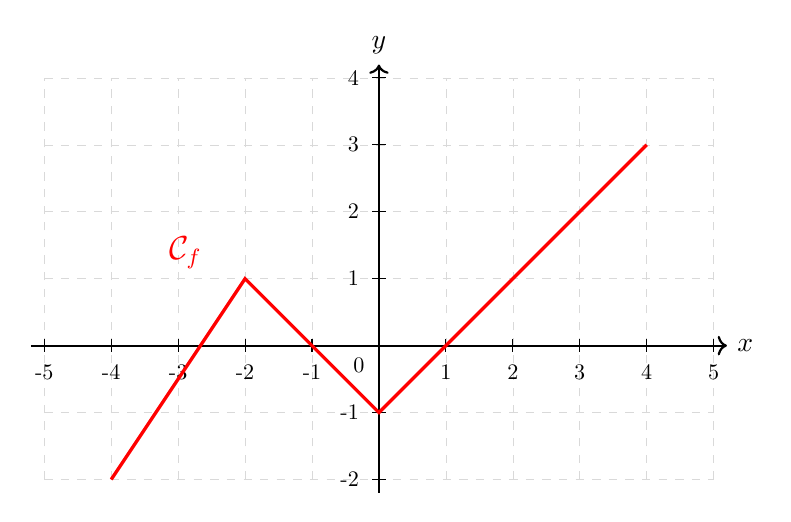
\begin{tikzpicture}[scale=0.85]
    % Grille et axes
    \draw[help lines, color=gray!30, dashed] (-5,-2) grid (5,4);
    \draw[->, thick] (-5.2,0) -- (5.2,0) node[right] {$x$};
    \draw[->, thick] (0,-2.2) -- (0,4.2) node[above] {$y$};

    % Graduations
    \foreach \x in {-5,-4,-3,-2,-1,1,2,3,4,5}
        \draw (\x, 0.1) -- (\x, -0.1) node[below=2pt, scale=0.8] {\x};
    \foreach \y in {-2,-1,1,2,3,4}
        \draw (0.1, \y) -- (-0.1, \y) node[left=2pt, scale=0.8] {\y};
    \node at (-0.3,-0.3) [scale=0.8] {0};

    % Courbe représentative (Cf)
    \draw[red, very thick] (-4,-2) -- (-2,1) -- (0,-1) -- (4,3);

    % Étiquette de la courbe
    \node[red, above left] at (-2.5, 1) {\large $\mathcal{C}_f$};
\end{tikzpicture}
\end{center}

\begin{enumerate}
    \item $f$ est-elle une application injective ? surjective ? bijective ? justifier vos réponses. \hfill \textbf{(0,5pt+0,5pt+0,5pt)}
    \item Quelles sont les images respectives des nombres $-4$ et $0$ ? \hfill \textbf{(0,25pt+0,25pt)}
    \item Quelle est l'image directe de l'intervalle $[-4; 0]$ ? \hfill \textbf{0,5pt}
    \item Donner l'image réciproque de l'intervalle $[-2; 1]$. \hfill \textbf{0,5pt}
\end{enumerate}

\vspace{0.3em}
\noindent\textbf{Partie B}

Soient $f$ et $g$ les applications définies par :
\[
f : \begin{array}[t]{rcl}
    ]1; +\infty[ & \to & \mathbb{R} \\
    x & \mapsto & \dfrac{2x}{x^2+1}
\end{array}
\quad \text{et} \quad
g : \begin{array}[t]{rcl}
    \mathbb{R} & \to & ]2; +\infty[ \\
    x & \mapsto & \dfrac{x+3}{x^2-1}
\end{array}
\]

\begin{enumerate}
    \item $f$ et $g$ sont-elles des applications ? justifier les réponses. \hfill \textbf{0,5pt + 0,5pt}
    \item Soit l'application $h$ définie par :
    \[
    h : \begin{array}[t]{rcl}
        ]1; +\infty[ & \to & ]2; +\infty[ \\
        x & \mapsto & \dfrac{2x + 1}{x - 1}
    \end{array}
    \]
    \begin{enumerate}
        \item Montrer que $h$ est injective. \hfill \textbf{0,75pt}
        \item Montrer que $h$ est surjective. \hfill \textbf{0,75pt}
        \item En déduire que $h$ est bijective puis donner l'expression de la bijection réciproque $h^{-1}$. \hfill \textbf{0,5pt + 0,5pt}
    \end{enumerate}
\end{enumerate}

\fbox{\textbf{\exo}}(2 points)

Soit l'application $\begin{array}[t]{rcl}
    f : \mathbb{R} & \longrightarrow & \mathbb{R} \\
    x & \longrightarrow & f(x) = 3 - |2 - x|.
\end{array}$

\begin{enumerate}
    \item Écrire $f$ sans le symbole valeur absolue. \hfill \textbf{(1 pt)}
    \item Déterminer la restriction $g$ de $f$ à l'intervalle $]-\infty ; 2]$. \hfill \textbf{(0.5 pt)}
    \item Déterminer la restriction $g$ de $f$ à l'intervalle $[2 ; +\infty[$. \hfill \textbf{(0.5 pt)}
\end{enumerate}

\fbox{\textbf{\exo}}(3,5 points)

Soit l'application $\begin{array}[t]{rcl}
    f : \mathbb{R} - \{1\} & \longrightarrow & \mathbb{R} - \{2\} \\
    x & \longrightarrow & f(x) = \frac{2x-3}{x-1}.
\end{array}$

\begin{enumerate}
    \item Démontrer que $f$ est injective et surjective. \hfill \textbf{(1.5 pts)}
    \item En déduire que $f$ est bijective. \hfill \textbf{(1 pt)}
    \item Déterminer la bijection réciproque $f^{-1}$. \hfill \textbf{(1 pt)}
\end{enumerate}

\fbox{\textbf{\exo}}(5,5 points)

Soit $f$ l'application dont la courbe $\mathcal{C}_f$ est donnée dans le repère orthonormal ci-après.

\begin{enumerate}
    \item Déterminer graphiquement l'image directe par $f$ de l'intervalle $[2; 5]$. \hfill \textbf{(1 pt)}
    \item Déterminer graphiquement l'image directe par $f$ des réels suivants : $-4$; $0$ et $2$. \hfill \textbf{(1.5 pts)}
    \item Déterminer graphiquement l'image réciproque par $f$ des réels suivants : $-3$; $-1$; $1$; $2{,}5$ \hfill \textbf{(2 pts)}
    \item Déterminer graphiquement l'image réciproque par $f$ de l'intervalle $[1; 3]$. \hfill \textbf{(1 pt)}
\end{enumerate}

\begin{center}
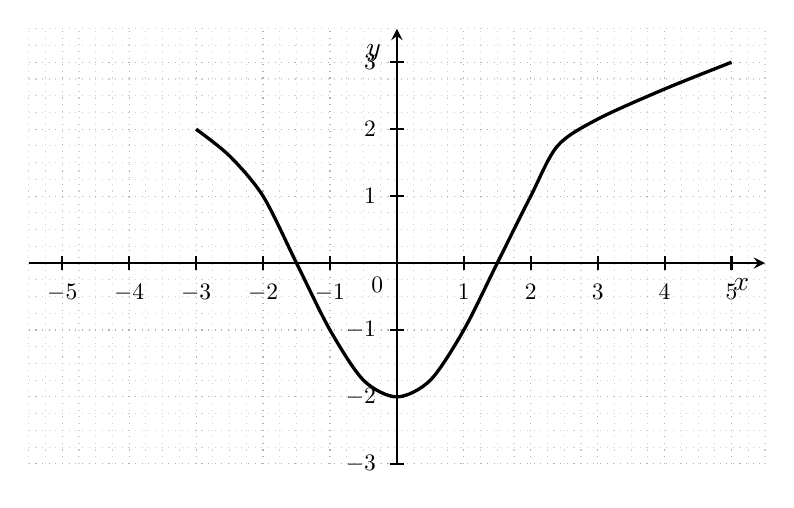
\begin{tikzpicture}[scale=0.85]
    % Grille secondaire (pas de 0.25) et principale (pas de 1)
    \draw[step=0.25cm, gray!35, dotted] (-5.5,-3) grid (5.5,3.5);
    \draw[step=1cm, gray!60, dotted] (-5.5,-3) grid (5.5,3.5);

    % Axes
    \draw[->, >=stealth, thick] (-5.5,0) -- (5.5,0) node[below left=2pt] {$x$};
    \draw[->, >=stealth, thick] (0,-3) -- (0,3.5) node[below left=2pt] {$y$};

    % Graduations sur l'axe des abscisses
    \foreach \x in {-5,-4,-3,-2,-1,1,2,3,4,5} {
        \draw[thick] (\x, 0.1) -- (\x, -0.1) node[below=2pt, scale=0.85] {$\x$};
    }
    \node[below left=2pt, scale=0.85] at (0,0) {$0$};

    % Graduations sur l'axe des ordonnées
    \foreach \y in {-3,-2,-1,1,2,3} {
        \draw[thick] (0.1, \y) -- (-0.1, \y) node[left=2pt, scale=0.85] {$\y$};
    }

    % Courbe représentative (Cf)
    \draw[very thick, smooth] plot coordinates {
        (-3, 2)
        (-2.5, 1.6)
        (-2, 1)
        (-1.5, 0)
        (-1, -1)
        (-0.5, -1.75)
        (0, -2)
        (0.5, -1.75)
        (1, -1)
        (1.5, 0)
        (2, 1)
        (2.4, 1.75)
        (3, 2.15)
        (4, 2.6)
        (5, 3)
    };
\end{tikzpicture}
\end{center}

\fbox{\textbf{\exo}}(6 points)

\begin{enumerate}
    \item On considère la correspondance $f$ de A vers B dont le diagramme sagittal est donnés ci-dessous :

    \begin{center}
    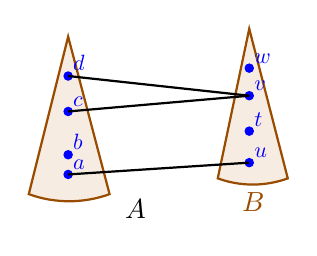
\begin{tikzpicture}[scale=1]
        % Ensemble A (forme conique)
        \draw[draw=orange!60!black, fill=orange!15!brown!15, thick] (0.5, 2.2) -- (0, 0.2) arc (250:290:1.5) -- cycle;
        \node[below right] at (1.1, 0.25) {$A$};

        % Points de l'ensemble A
        \filldraw[blue] (0.5, 1.7) circle (1.5pt) node[above right=-1pt, scale=0.8] {$d$};
        \filldraw[blue] (0.5, 1.25) circle (1.5pt) node[above right=-1pt, scale=0.8] {$c$};
        \filldraw[blue] (0.5, 0.7) circle (1.5pt) node[above right=-1pt, scale=0.8] {$b$};
        \filldraw[blue] (0.5, 0.45) circle (1.5pt) node[above right=-1pt, scale=0.8] {$a$};

        % Ensemble B (forme conique)
        \draw[draw=orange!60!black, fill=orange!15!brown!15, thick] (2.8, 2.3) -- (2.4, 0.4) arc (250:290:1.3) -- cycle;
        \node[below, orange!60!black] at (2.85, 0.35) {$B$};

        % Points de l'ensemble B
        \filldraw[blue] (2.8, 1.8) circle (1.5pt) node[above right=-1pt, scale=0.8] {$w$};
        \filldraw[blue] (2.8, 1.45) circle (1.5pt) node[above right=-1pt, scale=0.8] {$v$};
        \filldraw[blue] (2.8, 1.0) circle (1.5pt) node[above right=-1pt, scale=0.8] {$t$};
        \filldraw[blue] (2.8, 0.6) circle (1.5pt) node[above right=-1pt, scale=0.8] {$u$};

        % Flèches / Liens
        \draw[thick] (0.5, 1.7) -- (2.8, 1.45);
        \draw[thick] (0.5, 1.25) -- (2.8, 1.45);
        \draw[thick] (0.5, 0.45) -- (2.8, 0.6);
    \end{tikzpicture}
    \end{center}

    Expliquer pourquoi $f$ n'est pas une application de A vers B \hfill (1pt)

    \item E et F sont deux ensembles non vide\\
    Soit l'application $g$ définie de E vers F Compléter :
    \begin{enumerate}
        \item $g$ est une injection si \dotfill \hfill (1pt)
        \item $g$ est une surjection si \dotfill \hfill (1pt)
        \item $g$ est une bijection si \dotfill \hfill (1pt)
    \end{enumerate}

    \item Soit $h$ l'application dont sa courbe représentative est ci-dessous et soit $A = [-1; 2]$ et $B = [1; 4]$

    \begin{center}
    \begin{tikzpicture}[scale=0.8]
        % Axes
        \draw[->, >=stealth, thick] (-4.2, 0) -- (4.2, 0);
        \draw[->, >=stealth, thick] (0, -3.3) -- (0, 6.3);

        % Graduations X
        \foreach \x in {-4,-3,-2,-1,1,2,3,4} {
            \draw (\x, 0.08) -- (\x, -0.08) node[below, scale=0.75] {\x};
        }
        \node[above left, scale=0.75] at (0,0) {0};

        % Graduations Y
        \foreach \y in {-3,-2,-1,1,2,3,4,5,6} {
            \draw (0.08, \y) -- (-0.08, \y) node[left, scale=0.75] {\y};
        }

        % Courbe de h(x) = x^2
        \draw[thick, domain=-2.5:2.5, samples=100] plot (\x, {\x*\x});
        \node[right, scale=0.8] at (-2.4, 6) {h};
    \end{tikzpicture}
    \end{center}

    \begin{enumerate}
        \item Déterminer graphiquement l'image directe de $A$ par $h$ \hfill (1pt)
        \item Déterminer graphiquement l'image réciproque de $B$ par $h$ \hfill (1pt)
    \end{enumerate}
\end{enumerate}


\fbox{\textbf{\exo}}(4 points)

On considère la fonction suivante :
\[
\begin{array}{rcl}
    f : [-1 ; +\infty[ & \to & B \\
    x & \mapsto & x^2 + 2x - 3
\end{array}
\]

\begin{enumerate}
    \item[1)] Déterminer $B$ pour que $f$ soit bijective. \hfill \textbf{0,5 pt}
    \item[2)] Déterminer la bijection réciproque de $f$. \hfill \textbf{0,75pt}
    \item[3)] Soit l'application définie de $\mathbb{R}$ vers $\mathbb{R}$ par : $f(x) = |x^2 - 5x + 6|$\\
    Déterminer $g$ ; la restriction de $f$ à l'intervalle $[2 ; 3]$ \hfill \textbf{0,5pt}

    Soit $\begin{array}[t]{rcl}
        g : \mathbb{R} & \to & \mathbb{R} \\
        x & \mapsto & 2x + 5
    \end{array}$
    \item[4)] Déterminer l'image par $g$ de chacun des entiers : $-2$ ; $-1$ ; $2$. \hfill \textbf{0,75pt}
    \item[5)] Déterminer l'antécédent par $g$ de chacun des entiers $1$ ; $2$ et $3$. \hfill \textbf{0,75pt}
    \item[6)] L'application $g$ est-elle injective ? surjective ? bijective ? \hfill \textbf{(0,25+0,25+0,25) pts}
\end{enumerate}

\fbox{\textbf{\exo}}(3,5 points)

\begin{enumerate}
    \item[\textbf{1.}] Soit $h : \mathbb{R} \to \mathbb{R}$ par $h(x) = x^3 - x$. $h$ est-elle injective ? surjective ? \hfill \textbf{(01 \textit{point})}\\
    Déterminer $h^{-1}([-1; 1])$ et $f(\mathbb{R}^+)$. \hfill \textbf{(01 \textit{point})}

    \item[\textbf{2.}] On considère la $i$ définie sur $E = \mathbb{R} - \{1\}$ par : $i(x) = \frac{2x+1}{x-1}$. Montrer que $i$ réalise une bijection de $E\ \text{vers}\ i(E)$ à déterminer puis définir $i^{-1}$. \hfill \textbf{(01,5 \textit{point})}
\end{enumerate}


\fbox{\textbf{\exo}}(10 points)

\vspace{0.5em}

\noindent\underline{\textbf{Partie I :}}

\noindent Soit $f : \mathbb{R} \longrightarrow \mathbb{R}$ et $g : \mathbb{R} \longrightarrow \mathbb{R}_+$ de représentation graphique respectives $(\mathcal{C}_f)$ et $(\mathcal{C}_g)$ ci-dessous :

\begin{center}
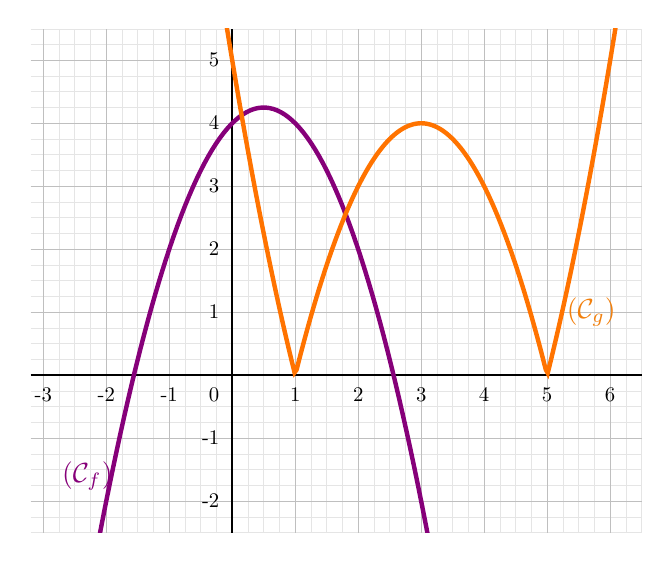
\begin{tikzpicture}[scale=0.8]
    % Grille secondaire (pas de 0.25) et principale (pas de 1)
    \draw[step=0.25cm, gray!20, very thin] (-3.2,-2.5) grid (6.5,5.5);
    \draw[step=1cm, gray!50, thin] (-3.2,-2.5) grid (6.5,5.5);

    % Axes
    \draw[thick] (-3.2,0) -- (6.5,0);
    \draw[thick] (0,-2.5) -- (0,5.5);

    % Graduations X
    \foreach \x in {-3,-2,-1,1,2,3,4,5,6} {
        \node[below=2pt, scale=0.75] at (\x, 0) {\x};
    }
    \node[below left=2pt, scale=0.75] at (0,0) {0};

    % Graduations Y
    \foreach \y in {-2,-1,1,2,3,4,5} {
        \node[left=2pt, scale=0.75] at (0, \y) {\y};
    }

    % Courbe (Cf) en violet : parabole passant par (-1,2), (0,4), (1,4), (2,2) -> y = -x^2 + x + 4
    \clip (-3.2,-2.5) rectangle (6.5,5.5);
    \draw[purple!70!blue, ultra thick, domain=-2.5:3.5, samples=100] plot (\x, {-\x*\x + \x + 4});
    \node[purple!70!blue] at (-2.3, -1.6) {$(\mathcal{C}_f)$};

    % Courbe (Cg) en orange : |-(x-3)^2 + 4| = |(x-1)(x-5)|
    \draw[orange!90!red, ultra thick, domain=-0.2:6.2, samples=200] plot (\x, {abs(-(\x-3)*(\x-3) + 4)});
    \node[orange!80!brown] at (5.7, 1) {$(\mathcal{C}_g)$};
\end{tikzpicture}
\end{center}

\begin{enumerate}
    \item[1)] $f\ \text{et}\ g$ sont-elles injectives ? surjectives ? bijectives ? justifier \hfill \underline{\textbf{01,5 pts}}
    \item[2)] Déterminer graphiquement :
    \begin{enumerate}
        \item[a)] $f(0), \quad f^{-1}(\{2\}), \quad g(3)\ \text{et}\ g^{-1}(\{0\})$ \hfill \underline{\textbf{01 pt}}
        \item[b)] $f([-1; 0]), \quad f^{-1}([5; +\infty[), \quad g(]0; 1])\ \text{et}\ g^{-1}(]-2; 0])$ \hfill \underline{\textbf{03 pts}}
    \end{enumerate}
    \item[3)] La restriction de $f$ sur l'intervalle $]-\infty; 0]$ est-elle bijective ? justifier. \hfill \underline{\textbf{01 pt}}
\end{enumerate}

\end{document}